\documentclass{article}

% Language setting
\usepackage[english]{babel}

% Page size and margins
\usepackage[letterpaper,top=2cm,bottom=2cm,left=3cm,right=3cm,marginparwidth=1.75cm]{geometry}

% Packages
\usepackage{amsmath,amssymb,amsthm}
\usepackage{color}
\usepackage{xcolor}
\usepackage{indentfirst}
\usepackage{graphicx}
\usepackage{makecell}
\usepackage{listings}
\usepackage{array}
\usepackage{mathpazo}
\usepackage{csquotes}

% Title font
\newcommand{\titlefont}{\fontfamily{ppl}\selectfont}

% Additional packages for formatting and boxes
\usepackage{titlesec}
\usepackage{colortbl}
\usepackage{multirow}
\usepackage{tabularx}
\usepackage[most]{tcolorbox}
\tcbuselibrary{many} % Can keep this, it loads common libraries
% \tcbuselibrary{skins, breakable, float}
\usepackage{subcaption}
\usepackage{soul} % For \hl
\usepackage{fancyhdr}
\usepackage{tikz}
\usepackage{mdframed}
\usepackage{enumitem}
\usepackage[colorlinks=true,allcolors=blue]{hyperref}
\usetikzlibrary{decorations,positioning,shapes.geometric,arrows.meta,fit,backgrounds,petri}

% Custom colors
\definecolor{codegreen}{rgb}{0,0.6,0}
\definecolor{codegray}{rgb}{0.5,0.5,0.5}
\definecolor{codepurple}{rgb}{0.58,0,0.82}
\definecolor{backcolour}{rgb}{0.95,0.95,0.92}

% Header/Footer
\pagestyle{fancy}
\fancyhead{}
\fancyfoot{}
\lhead{Instructor: Prof. Sharon Myers}
\rhead{How to Get Rid of a Botnet Infection.}
\lfoot{English 202C, Spring 2025, Instruction Guide}
\cfoot{\thepage}
\rfoot{UC Choudhary (ufc5009)}

\renewcommand{\footrulewidth}{0.4pt}

% Listings settings
\lstdefinestyle{mystyle}{
    backgroundcolor=\color{backcolour},
    commentstyle=\color{codegreen},
    keywordstyle=\color{magenta},
    numberstyle=\tiny\color{codegray},
    stringstyle=\color{codepurple},
    basicstyle=\ttfamily\footnotesize,
    breakatwhitespace=false,
    breaklines=true,
    captionpos=b,
    keepspaces=true,
    numbers=left,
    numbersep=5pt,
    showspaces=false,
    showstringspaces=false,
    showtabs=false,
    tabsize=2
}
\lstset{style=mystyle}


\lhead{Aditya Choudhary}
\rhead{Dhirubhai Ambani International School}

\lfoot{International Youth Math Challenge}
\cfoot{\thepage}
\rfoot{Qualification Round 2025}


\title{International Youth Math Challenge}
\author{Aditya Choudhary}
\date{}
\begin{document}
\maketitle
\thispagestyle{fancy}

\begin{figure}[h!]
    \centering
    \includegraphics[width=0.2\textwidth]{logo.png}
\end{figure}
\section*{Problem A}
\noindent A sequence is defined by $a_1 = 1$ and $a_{n+1} = a_n + n + 1$. Find a closed-form equation to calculate the value of $a_n$ and determine $a_{100}$.\\

\begin{tcolorbox}[
    colback=yellow!10,
    colframe=black!80!black,
    title={\textbf{Answer A}},
    fonttitle=\bfseries\large\centering,
    arc=4mm,
    boxrule=1pt,
    enhanced,
    breakable,
    overlay={
        % Repeat watermark across full box area
        \foreach \x in {-3,-2,-1,0,1,2,3}{
            \foreach \y in {-3,-2,-1,0,1,2,3}{
                \node[opacity=0.3, scale=1, text=black!20, rotate=45]
                    at ([xshift=\x*2cm, yshift=\y*1.2cm]frame.center)
                    {Aditya Choudhary};
            }
        }
    }
]

\begin{itemize}
    \item Key Ideas: Recurrence Relations, Discrete Math.
\end{itemize}

\noindent Given the recurrence 
\[
a_1 = 1,\qquad a_{n+1} = a_n + n + 1,
\]
rewriting $a_{n-1} + n$ as $1 + \sum_{k=1}^{n-1}(k+1)$\\
\[
\implies a_n = 1 + \sum_{k=1}^{n-1}(k+1)
    = 1 + \frac{(n-1)n}{2} + (n-1)
    = 1 + \frac{(n-1)(n+2)}{2}.
\]
Simplifying:
\[
a_n = \frac{n(n+1)}{2}.
\]
Hence
\[
a_{100} = \frac{100 \cdot 101}{2} = 5050.
\]

\[
\boxed{a_n=\tfrac{n(n+1)}{2},\quad a_{100}=5050.}
\]

\end{tcolorbox}

\hline
\newpage \section*{Problem B}
\noindent Show that there is no $x \in \mathbb{R}$ that solves the equation $\sqrt{3 + x} + \sqrt{7 - x} = 5$.\\
\begin{tcolorbox}[
    colback=yellow!10,
    colframe=black!80!black,
    title={\textbf{Answer B}},
    fonttitle=\bfseries\large\centering,
    arc=4mm,
    boxrule=1pt,
    enhanced,
    breakable,
    overlay={
        % Repeat watermark across full box area
        \foreach \x in {-3,-2,-1,0,1,2,3}{
            \foreach \y in {-3,-2,-1,0,1,2,3}{
                \node[opacity=0.3, scale=1, text=black!20, rotate=45]
                    at ([xshift=\x*2cm, yshift=\y*1.2cm]frame.center)
                    {Aditya Choudhary};
            }
        }
    }
]
\begin{itemize}
    \item Key Ideas: Quadratic Equations, \textit{\textbf{The Quadratic Equation}}, Properties of Discriminant.
    \item We know that, ``In a quadratic equation of the form $ax^2 + bx +c$ when $D=b^2-4ac$ is less than zero, \textit{x} has two imaginary roots."
\end{itemize}
\noindent Solve
\[
\sqrt{3+x}+\sqrt{7-x}=5.
\]
Let \(s=\sqrt{3+x}\), \(t=\sqrt{7-x}\), so \(s+t=5\).  
Then
\[
s^2+t^2=(3+x)+(7-x)=10.
\]
Square \(s+t=5\):
\[
10 + 2st = 25 \quad\Rightarrow\quad st=\frac{15}{2}.
\]
Square again:
\[
(3+x)(7-x)=\left(\frac{15}{2}\right)^2 = 56.25.
\]
Expand:
\[
21+4x-x^2 = 56.25.
\]
Thus
\[
x^2 - 4x + 35.25 = 0.
\]
The discriminant:
\[
D = (-4)^2 - 4(35.25) = 16 - 141 = -125 < 0.
\]
No real \(x\) satisfies the equation.

\[
\boxed{\text{No real solutions.}}
\]
\end{tcolorbox}

\hline
\newpage \section*{Problem C}
\noindent Determine the numerical value of the following expression without the use of a calculator:
\[
\sum_{k=1}^{3} \frac{\sin\left(\frac{k\pi}{12}\right) + \sin\left(\frac{(6-k)\pi}{12}\right)}{\cos\left(\frac{k\pi}{12}\right) + \cos\left(\frac{(6-k)\pi}{12}\right)} - \prod_{m=1}^{2} \frac{\tan\left(\frac{\pi}{4} + \frac{m\pi}{12}\right) - \tan\left(\frac{\pi}{4} - \frac{m\pi}{12}\right)}{1 + \tan\left(\frac{\pi}{4} + \frac{m\pi}{12}\right)\tan\left(\frac{\pi}{4} - \frac{m\pi}{12}\right)}
\]
\begin{tcolorbox}[
    colback=yellow!10,
    colframe=black!80!black,
    title={\textbf{Answer C}},
    fonttitle=\bfseries\large\centering,
    arc=4mm,
    boxrule=1pt,
    enhanced,
    breakable,
    overlay={
        % Repeat watermark across full box area
        \foreach \x in {-3,-2,-1,0,1,2,3}{
            \foreach \y in {-3,-2,-1,0,1,2,3}{
                \node[opacity=0.3, scale=1, text=black!20, rotate=45]
                    at ([xshift=\x*2cm, yshift=\y*1.2cm]frame.center)
                    {Aditya Choudhary};
            }
        }
    }
]
\begin{itemize}
    \item Key Ideas: Trigonometric Equations, \textit{\textbf{Trigonometric Transformations}},\\ Standard Trignometric Values for multiples of $\pi$.
\end{itemize}
\noindent Evaluate:
\[
\sum_{k=1}^{3}\frac{\sin\!\left(\frac{k\pi}{12}\right)+\sin\!\left(\frac{(6-k)\pi}{12}\right)}
{\cos\!\left(\frac{k\pi}{12}\right)+\cos\!\left(\frac{(6-k)\pi}{12}\right)}
-2\prod_{m=1}^{2}\frac{\tan\!\left(\frac{\pi}{4}+\frac{m\pi}{12}\right)-\tan\!\left(\frac{\pi}{4}-\frac{m\pi}{12}\right)}
{1+\tan\!\left(\frac{\pi}{4}+\frac{m\pi}{12}\right)\tan\!\left(\frac{\pi}{4}-\frac{m\pi}{12}\right)}.
\]

\noindent For the second term, using the identity:
\[
\frac{\tan A-\tan B}{1+\tan A\tan B} = \tan(A-B).
\]
where \[
A = \left(\frac{\pi}{4}+\frac{m\pi}{12}\right), \hspace{20pt}
B=\left(\frac{\pi}{4}-\frac{m\pi}{12}\right)
\]
Thus the product \(-2\prod_{m=1}^{2}\frac{\tan\!\left(\frac{\pi}{4}+\frac{m\pi}{12}\right)-\tan\!\left(\frac{\pi}{4}-\frac{m\pi}{12}\right)}
{1+\tan\!\left(\frac{\pi}{4}+\frac{m\pi}{12}\right)\tan\!\left(\frac{\pi}{4}-\frac{m\pi}{12}\right)}\). becomes
\[
\prod_{m=1}^2 \tan\left(\frac{m\pi}{6}\right)
= \tan\left(\frac{\pi}{6}\right)\tan\left(\frac{\pi}{3}\right)
= \frac{1}{\sqrt{3}}\cdot \sqrt{3}=1.
\]
So the second term is \(\boxed{-2\prod_{m=1}^{2}\frac{\tan\!\left(\frac{\pi}{4}+\frac{m\pi}{12}\right)-\tan\!\left(\frac{\pi}{4}-\frac{m\pi}{12}\right)}
{1+\tan\!\left(\frac{\pi}{4}+\frac{m\pi}{12}\right)\tan\!\left(\frac{\pi}{4}-\frac{m\pi}{12}\right)} =(-2)}\).\\
\hline
\vspace{15pt}
\noindent Next simplifying:\\
\[\implies
\frac{(6-k)\pi}{12} = \frac{\pi}{2}-\frac{k\pi}{12}.
\]
Hence since sine and cosine are complementary.  
\[
\sin\!\left(\frac{(6-k)\pi}{12}\right)=\cos\!\left(\frac{k\pi}{12}\right),\qquad
\cos\!\left(\frac{(6-k)\pi}{12}\right)=\sin\!\left(\frac{k\pi}{12}\right).
\]
Thus each summand becomes
\[
\frac{\sin\theta+\cos\theta}{\cos\theta+\sin\theta}=1. \hspace{10pt}
\because \text{substituting }\theta = \frac{k\pi}{12}
\]
Summing \(\sum_{k=1}^{3} \frac{\sin\left(\frac{k\pi}{12}\right) + \sin\left(\frac{(6-k)\pi}{12}\right)}{\cos\left(\frac{k\pi}{12}\right) + \cos\left(\frac{(6-k)\pi}{12}\right)}\) gives \(3 \hspace{10pt} (\because \sum = 1\times3)\).  \\
Therefore:
\[
\boxed{3 - 2 = 1.}
\]
\end{tcolorbox}

\hline
\newpage \section*{Problem D}
\noindent Prove that for every positive integer $n$, the number $n^4 + 4$ is a composite number, except for one value of $n$.
\begin{tcolorbox}[
    colback=yellow!10,
    colframe=black!80!black,
    title={\textbf{Answer D}},
    fonttitle=\bfseries\large\centering,
    arc=4mm,
    boxrule=1pt,
    enhanced,
    breakable,
    overlay={
        % Repeat watermark across full box area
        \foreach \x in {-3,-2,-1,0,1,2,3}{
            \foreach \y in {-3,-2,-1,0,1,2,3}{
                \node[opacity=0.3, scale=1, text=black!20, rotate=45]
                    at ([xshift=\x*2cm, yshift=\y*1.2cm]frame.center)
                    {Aditya Choudhary};
            }
        }
    }
]
\begin{itemize}
    \item Key Ideas: Sophie Germain's identity, \textit{\textbf{Number Theory}}.\\
    \item ``A number is prime when it is divisible only by 1 and itself." \textbf{\textit{\hl{In other words, if both factors are greater than 1, the number is composite.}}}
\end{itemize}
\noindent\textbf{\underline{Claim:}} For every positive integer \(n\), the integer \(n^4+4\) is composite, except when \(n=1\) (in which case \(n^4+4=5\) is prime).

\begin{proof}
We begin by exhibiting an integer factorization of \(n^4+4\). Observe that
\[
n^4+4 = n^4 + 4n^2 + 4 - 4n^2 = (n^2+2)^2 - (2n)^2,
\]
from Sophie Germain's identity, so \(n^4+4\) is a difference of squares and therefore factors as
\[
n^4+4 = \big(n^2+2 - 2n\big)\big(n^2+2 + 2n\big).
\]
Rewriting each factor in a convenient form yields
\[
n^2 - 2n + 2 \qquad\text{and}\qquad n^2 + 2n + 2.
\]
Both factors are integers \(\forall n \in \mathbb{Z}\), hence this is a valid factorization in \(\mathbb{Z}\).

It remains to show that for positive integers \(n\) with \(n\ge 2\) both factors are strictly greater than \(1\). Note that
\[
n^2 - 2n + 2 = (n-1)^2 + 1 \quad\text{and}\quad n^2 + 2n + 2 = (n+1)^2 + 1.
\]
If \(n\ge 2\) then \((n-1)^2 \ge 1\), so
\[
n^2 - 2n + 2 = (n-1)^2 + 1 \ge 1 + 1 = 2.
\]
Similarly, for every \(n\ge 1\) we have \((n+1)^2\ge 4\), so \(n^2+2n+2=(n+1)^2+1\ge 5>1\). Thus for \(n\ge 2\) both factors exceed \(1\), and therefore \(n^4+4\) is the product of two integers greater than \(1\); in other words \(n^4+4\) is composite.

Finally, check the exceptional small value \(n=1\):
\[
1^4 + 4 = 5,
\]
which is prime. (For completeness, \(n=0\) yields \(0^4+4=4\), which is composite, but the statement concerns positive integers, not non-negative integers to which 0 belongs.)

Combining the above observations we conclude that \(n^4+4\) is composite for every positive integer \(n\ge 2\), with the sole exception \(n=1\), for which \(n^4+4\) is prime.\\
\textbf{Q.E.D}
\end{proof}
\end{tcolorbox}

\hline
\newpage
\section*{Problem E}

\noindent A rectangle with side lengths a and b is cut by a diagonal as shown in the drawing below. Find the perimeter and the area of the two triangles formed.
\vspace{10pt}
\begin{center}
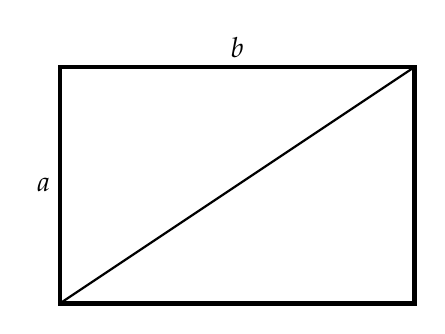
\begin{tikzpicture}[scale=1.5]
    % Draw rectangle
    \draw[ultra thick] (0,0) -- (3,0) -- (3,2) -- (0,2) -- cycle;
    % Draw diagonal
    \draw[thick] (0,0) -- (3,2);
    % Labels
    \node[above] at (1.5,2) {$b$};
    \node[left] at (0,1) {$a$};
\end{tikzpicture}
\end{center}

\begin{tcolorbox}[
    colback=yellow!10,
    colframe=black!80!black,
    title={\textbf{Answer E}},
    fonttitle=\bfseries\large\centering,
    arc=4mm,
    boxrule=1pt,
    enhanced,
    breakable,
    overlay={
        % Repeat watermark across full box area
        \foreach \x in {-3,-2,-1,0,1,2,3}{
            \foreach \y in {-3,-2,-1,0,1,2,3}{
                \node[opacity=0.3, scale=1, text=black!20, rotate=45]
                    at ([xshift=\x*2cm, yshift=\y*1.2cm]frame.center)
                    {Aditya Choudhary};
            }
        }
    }
]
\begin{itemize}
    \item Key Ideas: Quadrilateral, \textbf{\textit{Triangles}}
\end{itemize}
By RHS congruency, the two triangles formed by the diagonal are necessarily \emph{congruent}. It therefore suffices to compute the area and perimeter of one of the triangles.\\
The diagonal of the rectangle becomes the hypotenuse of the right triangle. By the Pythagorean theorem, which states that for any right triangle with legs \(x\) and \(y\) and hypotenuse \(z\),
\[
z^2 = x^2 + y^2,
\]
Taking the positive square root (since lengths are positive scalars), the hypotenuse is
\[
\boxed{c = \sqrt{a^2 + b^2}}.
\]

The area \(A\) of a right triangle with legs \(x\) and \(y\) is given by the standard formula
\[
A = \frac{1}{2}xy.
\]
Here the legs are \(a\) and \(b\). Therefore the area of each triangular piece after the rectangle is cut along its diagonal is
\[
A = \frac{1}{2}ab.
\]
Hence,
\[
\boxed{\text{Area of each triangle} = \tfrac{1}{2}ab}.
\]


The perimeter \(P\) of a triangle is defined as the sum of the lengths of its three sides. For our right triangle, the three side lengths are:
\[
a,\qquad b,\qquad \sqrt{a^2 + b^2}.
\]
Therefore,
\[
P = a + b + \sqrt{a^2 + b^2}.
\]
Thus,
\[
\boxed{\text{Perimeter of each triangle} = a + b + \sqrt{a^2 + b^2}}.
\]
\end{tcolorbox}
\begin{figure}[h!]
    \centering
    \includegraphics[width=0.4\linewidth]{end.jpg}
\end{figure}


\end{document}
